\documentclass[1p]{elsarticle_modified}
%\bibliographystyle{elsarticle-num}

%\usepackage[colorlinks]{hyperref}
%\usepackage{abbrmath_seonhwa} %\Abb, \Ascr, \Acal ,\Abf, \Afrak
\usepackage{amsfonts}
\usepackage{amssymb}
\usepackage{amsmath}
\usepackage{amsthm}
\usepackage{scalefnt}
\usepackage{amsbsy}
\usepackage{kotex}
\usepackage{caption}
\usepackage{subfig}
\usepackage{color}
\usepackage{graphicx}
\usepackage{xcolor} %% white, black, red, green, blue, cyan, magenta, yellow
\usepackage{float}
\usepackage{setspace}
\usepackage{hyperref}

\usepackage{tikz}
\usetikzlibrary{arrows}

\usepackage{multirow}
\usepackage{array} % fixed length table
\usepackage{hhline}

%%%%%%%%%%%%%%%%%%%%%
\makeatletter
\renewcommand*\env@matrix[1][\arraystretch]{%
	\edef\arraystretch{#1}%
	\hskip -\arraycolsep
	\let\@ifnextchar\new@ifnextchar
	\array{*\c@MaxMatrixCols c}}
\makeatother %https://tex.stackexchange.com/questions/14071/how-can-i-increase-the-line-spacing-in-a-matrix
%%%%%%%%%%%%%%%

\usepackage[normalem]{ulem}

\newcommand{\msout}[1]{\ifmmode\text{\sout{\ensuremath{#1}}}\else\sout{#1}\fi}
%SOURCE: \msout is \stkout macro in https://tex.stackexchange.com/questions/20609/strikeout-in-math-mode

\newcommand{\cancel}[1]{
	\ifmmode
	{\color{red}\msout{#1}}
	\else
	{\color{red}\sout{#1}}
	\fi
}

\newcommand{\add}[1]{
	{\color{blue}\uwave{#1}}
}

\newcommand{\replace}[2]{
	\ifmmode
	{\color{red}\msout{#1}}{\color{blue}\uwave{#2}}
	\else
	{\color{red}\sout{#1}}{\color{blue}\uwave{#2}}
	\fi
}

\newcommand{\Sol}{\mathcal{S}} %segment
\newcommand{\D}{D} %diagram
\newcommand{\A}{\mathcal{A}} %arc


%%%%%%%%%%%%%%%%%%%%%%%%%%%%%5 test

\def\sl{\operatorname{\textup{SL}}(2,\Cbb)}
\def\psl{\operatorname{\textup{PSL}}(2,\Cbb)}
\def\quan{\mkern 1mu \triangleright \mkern 1mu}

\theoremstyle{definition}
\newtheorem{thm}{Theorem}[section]
\newtheorem{prop}[thm]{Proposition}
\newtheorem{lem}[thm]{Lemma}
\newtheorem{ques}[thm]{Question}
\newtheorem{cor}[thm]{Corollary}
\newtheorem{defn}[thm]{Definition}
\newtheorem{exam}[thm]{Example}
\newtheorem{rmk}[thm]{Remark}
\newtheorem{alg}[thm]{Algorithm}

\newcommand{\I}{\sqrt{-1}}
\begin{document}

%\begin{frontmatter}
%
%\title{Boundary parabolic representations of knots up to 8 crossings}
%
%%% Group authors per affiliation:
%\author{Yunhi Cho} 
%\address{Department of Mathematics, University of Seoul, Seoul, Korea}
%\ead{yhcho@uos.ac.kr}
%
%
%\author{Seonhwa Kim} %\fnref{s_kim}}
%\address{Center for Geometry and Physics, Institute for Basic Science, Pohang, 37673, Korea}
%\ead{ryeona17@ibs.re.kr}
%
%\author{Hyuk Kim}
%\address{Department of Mathematical Sciences, Seoul National University, Seoul 08826, Korea}
%\ead{hyukkim@snu.ac.kr}
%
%\author{Seokbeom Yoon}
%\address{Department of Mathematical Sciences, Seoul National University, Seoul, 08826,  Korea}
%\ead{sbyoon15@snu.ac.kr}
%
%\begin{abstract}
%We find all boundary parabolic representation of knots up to 8 crossings.
%
%\end{abstract}
%\begin{keyword}
%    \MSC[2010] 57M25 
%\end{keyword}
%
%\end{frontmatter}

%\linenumbers
%\tableofcontents
%
\newcommand\colored[1]{\textcolor{white}{\rule[-0.35ex]{0.8em}{1.4ex}}\kern-0.8em\color{red} #1}%
%\newcommand\colored[1]{\textcolor{white}{ #1}\kern-2.17ex	\textcolor{white}{ #1}\kern-1.81ex	\textcolor{white}{ #1}\kern-2.15ex\color{red}#1	}

{\Large $\underline{12a_{0380}~(K12a_{0380})}$}

\setlength{\tabcolsep}{10pt}
\renewcommand{\arraystretch}{1.6}
\vspace{1cm}\begin{tabular}{m{100pt}>{\centering\arraybackslash}m{274pt}}
\multirow{5}{120pt}{
	\centering
	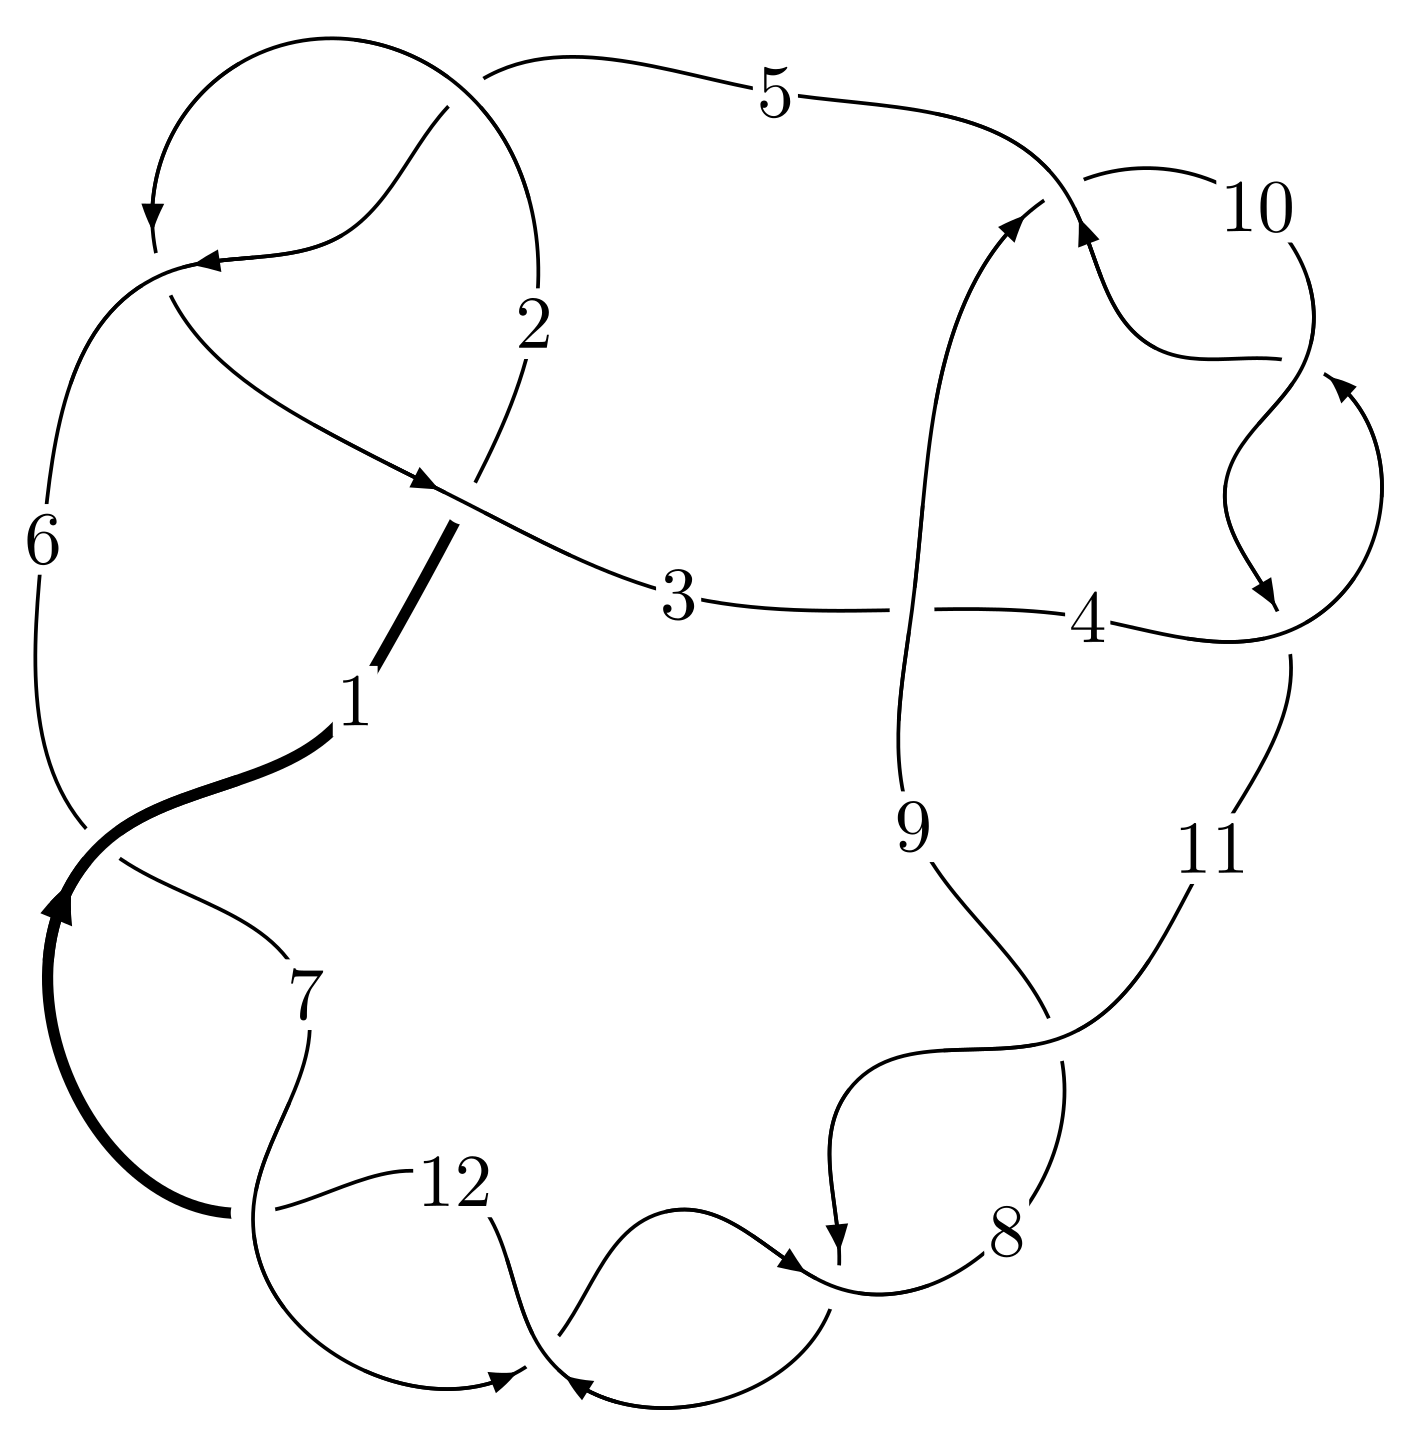
\includegraphics[width=112pt]{../../../GIT/diagram.site/Diagrams/png/1181_12a_0380.png}\\
\ \ \ A knot diagram\footnotemark}&
\allowdisplaybreaks
\textbf{Linearized knot diagam} \\
\cline{2-2}
 &
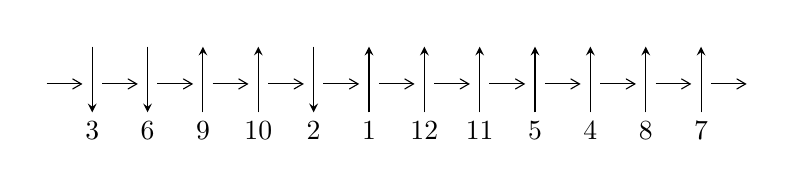
\begin{tikzpicture}[x=20pt, y=17pt]
	% nodes
	\node (C0) at (0, 0) {};
	\node (C1) at (1, 0) {};
	\node (C1U) at (1, +1) {};
	\node (C1D) at (1, -1) {3};

	\node (C2) at (2, 0) {};
	\node (C2U) at (2, +1) {};
	\node (C2D) at (2, -1) {6};

	\node (C3) at (3, 0) {};
	\node (C3U) at (3, +1) {};
	\node (C3D) at (3, -1) {9};

	\node (C4) at (4, 0) {};
	\node (C4U) at (4, +1) {};
	\node (C4D) at (4, -1) {10};

	\node (C5) at (5, 0) {};
	\node (C5U) at (5, +1) {};
	\node (C5D) at (5, -1) {2};

	\node (C6) at (6, 0) {};
	\node (C6U) at (6, +1) {};
	\node (C6D) at (6, -1) {1};

	\node (C7) at (7, 0) {};
	\node (C7U) at (7, +1) {};
	\node (C7D) at (7, -1) {12};

	\node (C8) at (8, 0) {};
	\node (C8U) at (8, +1) {};
	\node (C8D) at (8, -1) {11};

	\node (C9) at (9, 0) {};
	\node (C9U) at (9, +1) {};
	\node (C9D) at (9, -1) {5};

	\node (C10) at (10, 0) {};
	\node (C10U) at (10, +1) {};
	\node (C10D) at (10, -1) {4};

	\node (C11) at (11, 0) {};
	\node (C11U) at (11, +1) {};
	\node (C11D) at (11, -1) {8};

	\node (C12) at (12, 0) {};
	\node (C12U) at (12, +1) {};
	\node (C12D) at (12, -1) {7};
	\node (C13) at (13, 0) {};

	% arrows
	\draw[->,>={angle 60}]
	(C0) edge (C1) (C1) edge (C2) (C2) edge (C3) (C3) edge (C4) (C4) edge (C5) (C5) edge (C6) (C6) edge (C7) (C7) edge (C8) (C8) edge (C9) (C9) edge (C10) (C10) edge (C11) (C11) edge (C12) (C12) edge (C13) ;	\draw[->,>=stealth]
	(C1U) edge (C1D) (C2U) edge (C2D) (C3D) edge (C3U) (C4D) edge (C4U) (C5U) edge (C5D) (C6D) edge (C6U) (C7D) edge (C7U) (C8D) edge (C8U) (C9D) edge (C9U) (C10D) edge (C10U) (C11D) edge (C11U) (C12D) edge (C12U) ;
	\end{tikzpicture} \\
\hhline{~~} \\& 
\textbf{Solving Sequence} \\ \cline{2-2} 
 &
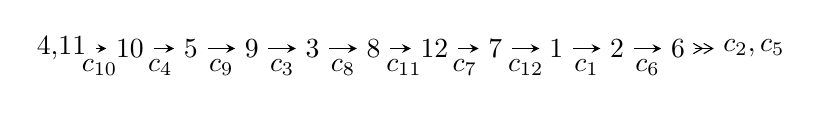
\begin{tikzpicture}[x=22pt, y=7pt]
	% node
	\node (A0) at (-1/8, 0) {4,11};
	\node (A1) at (1, 0) {10};
	\node (A2) at (2, 0) {5};
	\node (A3) at (3, 0) {9};
	\node (A4) at (4, 0) {3};
	\node (A5) at (5, 0) {8};
	\node (A6) at (6, 0) {12};
	\node (A7) at (7, 0) {7};
	\node (A8) at (8, 0) {1};
	\node (A9) at (9, 0) {2};
	\node (A10) at (10, 0) {6};
	\node (C1) at (1/2, -1) {$c_{10}$};
	\node (C2) at (3/2, -1) {$c_{4}$};
	\node (C3) at (5/2, -1) {$c_{9}$};
	\node (C4) at (7/2, -1) {$c_{3}$};
	\node (C5) at (9/2, -1) {$c_{8}$};
	\node (C6) at (11/2, -1) {$c_{11}$};
	\node (C7) at (13/2, -1) {$c_{7}$};
	\node (C8) at (15/2, -1) {$c_{12}$};
	\node (C9) at (17/2, -1) {$c_{1}$};
	\node (C10) at (19/2, -1) {$c_{6}$};
	\node (A11) at (45/4, 0) {$c_{2},c_{5}$};

	% edge
	\draw[->,>=stealth]	
	(A0) edge (A1) (A1) edge (A2) (A2) edge (A3) (A3) edge (A4) (A4) edge (A5) (A5) edge (A6) (A6) edge (A7) (A7) edge (A8) (A8) edge (A9) (A9) edge (A10) ;
	\draw[->>,>={angle 60}]	
	(A10) edge (A11);
\end{tikzpicture} \\ 

\end{tabular} \\

\footnotetext{
The image of knot diagram is generated by the software ``\textbf{Draw programme}" developed by Andrew Bartholomew(\url{http://www.layer8.co.uk/maths/draw/index.htm\#Running-draw}), where we modified some parts for our purpose(\url{https://github.com/CATsTAILs/LinksPainter}).
}\phantom \\ \newline 
\centering \textbf{Ideals for irreducible components\footnotemark of $X_{\text{par}}$} 
 
\begin{align*}
I^u_{1}&=\langle 
u^{38}+u^{37}+\cdots+u+1\rangle \\
\\
\end{align*}
\raggedright * 1 irreducible components of $\dim_{\mathbb{C}}=0$, with total 38 representations.\\
\footnotetext{All coefficients of polynomials are rational numbers. But the coefficients are sometimes approximated in decimal forms when there is not enough margin.}
\newpage
\renewcommand{\arraystretch}{1}
\centering \section*{I. $I^u_{1}= \langle u^{38}+u^{37}+\cdots+u+1 \rangle$}
\flushleft \textbf{(i) Arc colorings}\\
\begin{tabular}{m{7pt} m{180pt} m{7pt} m{180pt} }
\flushright $a_{4}=$&$\begin{pmatrix}0\\u\end{pmatrix}$ \\
\flushright $a_{11}=$&$\begin{pmatrix}1\\0\end{pmatrix}$ \\
\flushright $a_{10}=$&$\begin{pmatrix}1\\u^2\end{pmatrix}$ \\
\flushright $a_{5}=$&$\begin{pmatrix}u\\u^3+u\end{pmatrix}$ \\
\flushright $a_{9}=$&$\begin{pmatrix}u^2+1\\u^4+2 u^2\end{pmatrix}$ \\
\flushright $a_{3}=$&$\begin{pmatrix}- u^5-2 u^3- u\\- u^7-3 u^5-2 u^3+u\end{pmatrix}$ \\
\flushright $a_{8}=$&$\begin{pmatrix}- u^4- u^2+1\\u^4+2 u^2\end{pmatrix}$ \\
\flushright $a_{12}=$&$\begin{pmatrix}u^8+3 u^6+u^4-2 u^2+1\\- u^8-4 u^6-4 u^4\end{pmatrix}$ \\
\flushright $a_{7}=$&$\begin{pmatrix}- u^{12}-5 u^{10}-7 u^8+2 u^4-3 u^2+1\\u^{12}+6 u^{10}+12 u^8+8 u^6+u^4+2 u^2\end{pmatrix}$ \\
\flushright $a_{1}=$&$\begin{pmatrix}u^{16}+7 u^{14}+17 u^{12}+14 u^{10}- u^8+2 u^6+6 u^4-4 u^2+1\\- u^{16}-8 u^{14}-24 u^{12}-32 u^{10}-18 u^8-8 u^6-8 u^4\end{pmatrix}$ \\
\flushright $a_{2}=$&$\begin{pmatrix}u^{28}+13 u^{26}+\cdots-5 u^2+1\\u^{30}+14 u^{28}+\cdots-16 u^4+u^2\end{pmatrix}$ \\
\flushright $a_{6}=$&$\begin{pmatrix}- u^{20}-9 u^{18}+\cdots-5 u^2+1\\u^{20}+10 u^{18}+40 u^{16}+80 u^{14}+83 u^{12}+50 u^{10}+36 u^8+24 u^6+u^4+2 u^2\end{pmatrix}$\\&\end{tabular}
\flushleft \textbf{(ii) Obstruction class $= -1$}\\~\\
\flushleft \textbf{(iii) Cusp Shapes $= -4 u^{36}-4 u^{35}-72 u^{34}-68 u^{33}-580 u^{32}-516 u^{31}-2748 u^{30}-2292 u^{29}-8476 u^{28}-6576 u^{27}-17864 u^{26}-12736 u^{25}-26568 u^{24}-17112 u^{23}-29228 u^{22}-16736 u^{21}-26160 u^{20}-13388 u^{19}-21072 u^{18}-9832 u^{17}-14636 u^{16}-5896 u^{15}-7812 u^{14}-2336 u^{13}-3700 u^{12}-856 u^{11}-1816 u^{10}-336 u^9-456 u^8+80 u^7-56 u^6+40 u^5-68 u^4+20 u^3+24 u^2+16 u+2$}\\~\\
\newpage\renewcommand{\arraystretch}{1}
\flushleft \textbf{(iv) u-Polynomials at the component}\newline \\
\begin{tabular}{m{50pt}|m{274pt}}
Crossings & \hspace{64pt}u-Polynomials at each crossing \\
\hline $$\begin{aligned}c_{1}\end{aligned}$$&$\begin{aligned}
&u^{38}+23 u^{37}+\cdots+5 u+1
\end{aligned}$\\
\hline $$\begin{aligned}c_{2},c_{5}\end{aligned}$$&$\begin{aligned}
&u^{38}+u^{37}+\cdots+u+1
\end{aligned}$\\
\hline $$\begin{aligned}c_{3}\end{aligned}$$&$\begin{aligned}
&u^{38}- u^{37}+\cdots+81 u+317
\end{aligned}$\\
\hline $$\begin{aligned}c_{4},c_{9},c_{10}\end{aligned}$$&$\begin{aligned}
&u^{38}+u^{37}+\cdots+u+1
\end{aligned}$\\
\hline $$\begin{aligned}c_{6},c_{7},c_{8}\\c_{11},c_{12}\end{aligned}$$&$\begin{aligned}
&u^{38}+3 u^{37}+\cdots+15 u+3
\end{aligned}$\\
\hline
\end{tabular}\\~\\
\newpage\renewcommand{\arraystretch}{1}
\flushleft \textbf{(v) Riley Polynomials at the component}\newline \\
\begin{tabular}{m{50pt}|m{274pt}}
Crossings & \hspace{64pt}Riley Polynomials at each crossing \\
\hline $$\begin{aligned}c_{1}\end{aligned}$$&$\begin{aligned}
&y^{38}-15 y^{37}+\cdots+3 y+1
\end{aligned}$\\
\hline $$\begin{aligned}c_{2},c_{5}\end{aligned}$$&$\begin{aligned}
&y^{38}-23 y^{37}+\cdots-5 y+1
\end{aligned}$\\
\hline $$\begin{aligned}c_{3}\end{aligned}$$&$\begin{aligned}
&y^{38}+25 y^{37}+\cdots+1416135 y+100489
\end{aligned}$\\
\hline $$\begin{aligned}c_{4},c_{9},c_{10}\end{aligned}$$&$\begin{aligned}
&y^{38}+37 y^{37}+\cdots-5 y+1
\end{aligned}$\\
\hline $$\begin{aligned}c_{6},c_{7},c_{8}\\c_{11},c_{12}\end{aligned}$$&$\begin{aligned}
&y^{38}+53 y^{37}+\cdots+123 y+9
\end{aligned}$\\
\hline
\end{tabular}\\~\\
\newpage\flushleft \textbf{(vi) Complex Volumes and Cusp Shapes}
$$\begin{array}{c|c|c}  
\text{Solutions to }I^u_{1}& \I (\text{vol} + \sqrt{-1}CS) & \text{Cusp shape}\\
 \hline 
\begin{aligned}
u &= -0.699030 + 0.516783 I\end{aligned}
 & -16.5834 + 2.6642 I & -1.43407 - 0.13323 I \\ \hline\begin{aligned}
u &= -0.699030 - 0.516783 I\end{aligned}
 & -16.5834 - 2.6642 I & -1.43407 + 0.13323 I \\ \hline\begin{aligned}
u &= -0.709471 + 0.500003 I\end{aligned}
 & -16.5259 - 7.3585 I & -1.27138 + 5.67363 I \\ \hline\begin{aligned}
u &= -0.709471 - 0.500003 I\end{aligned}
 & -16.5259 + 7.3585 I & -1.27138 - 5.67363 I \\ \hline\begin{aligned}
u &= \phantom{-}0.699159 + 0.504973 I\end{aligned}
 & -12.61000 + 2.32929 I & \phantom{-}1.79922 - 2.79577 I \\ \hline\begin{aligned}
u &= \phantom{-}0.699159 - 0.504973 I\end{aligned}
 & -12.61000 - 2.32929 I & \phantom{-}1.79922 + 2.79577 I \\ \hline\begin{aligned}
u &= \phantom{-}0.046655 + 1.266040 I\end{aligned}
 & -2.65817 + 1.73113 I & \phantom{-}5.04604 - 4.55747 I \\ \hline\begin{aligned}
u &= \phantom{-}0.046655 - 1.266040 I\end{aligned}
 & -2.65817 - 1.73113 I & \phantom{-}5.04604 + 4.55747 I \\ \hline\begin{aligned}
u &= \phantom{-}0.617788 + 0.394340 I\end{aligned}
 & -5.75531 + 5.89610 I & -0.12847 - 7.53727 I \\ \hline\begin{aligned}
u &= \phantom{-}0.617788 - 0.394340 I\end{aligned}
 & -5.75531 - 5.89610 I & -0.12847 + 7.53727 I \\ \hline\begin{aligned}
u &= \phantom{-}0.548294 + 0.475497 I\end{aligned}
 & -6.07647 - 2.03534 I & -1.49342 + 0.25635 I \\ \hline\begin{aligned}
u &= \phantom{-}0.548294 - 0.475497 I\end{aligned}
 & -6.07647 + 2.03534 I & -1.49342 - 0.25635 I \\ \hline\begin{aligned}
u &= -0.553289 + 0.398678 I\end{aligned}
 & -2.61813 - 1.78595 I & \phantom{-}2.96437 + 4.13592 I \\ \hline\begin{aligned}
u &= -0.553289 - 0.398678 I\end{aligned}
 & -2.61813 + 1.78595 I & \phantom{-}2.96437 - 4.13592 I \\ \hline\begin{aligned}
u &= \phantom{-}0.108014 + 1.329890 I\end{aligned}
 & -3.47258 + 1.99659 I & \phantom{-}3.63851 - 3.32884 I \\ \hline\begin{aligned}
u &= \phantom{-}0.108014 - 1.329890 I\end{aligned}
 & -3.47258 - 1.99659 I & \phantom{-}3.63851 + 3.32884 I \\ \hline\begin{aligned}
u &= -0.165337 + 1.349130 I\end{aligned}
 & -5.18486 - 5.72137 I & \phantom{-0.000000 -}0. + 8.45786 I \\ \hline\begin{aligned}
u &= -0.165337 - 1.349130 I\end{aligned}
 & -5.18486 + 5.72137 I & \phantom{-0.000000 } 0. - 8.45786 I \\ \hline\begin{aligned}
u &= -0.070878 + 1.410250 I\end{aligned}
 & -7.16634 - 0.25397 I & \phantom{-0.000000 } 0 \\ \hline\begin{aligned}
u &= -0.070878 - 1.410250 I\end{aligned}
 & -7.16634 + 0.25397 I & \phantom{-0.000000 } 0 \\ \hline\begin{aligned}
u &= -0.529018 + 0.191801 I\end{aligned}
 & -0.35654 - 3.20662 I & \phantom{-}5.93778 + 9.20174 I \\ \hline\begin{aligned}
u &= -0.529018 - 0.191801 I\end{aligned}
 & -0.35654 + 3.20662 I & \phantom{-}5.93778 - 9.20174 I \\ \hline\begin{aligned}
u &= -0.19412 + 1.44071 I\end{aligned}
 & -8.51769 - 4.51489 I & \phantom{-0.000000 } 0 \\ \hline\begin{aligned}
u &= -0.19412 - 1.44071 I\end{aligned}
 & -8.51769 + 4.51489 I & \phantom{-0.000000 } 0 \\ \hline\begin{aligned}
u &= \phantom{-}0.21879 + 1.44502 I\end{aligned}
 & -11.6645 + 8.9374 I & \phantom{-0.000000 } 0 \\ \hline\begin{aligned}
u &= \phantom{-}0.21879 - 1.44502 I\end{aligned}
 & -11.6645 - 8.9374 I & \phantom{-0.000000 } 0 \\ \hline\begin{aligned}
u &= \phantom{-}0.18046 + 1.46649 I\end{aligned}
 & -12.33810 + 0.59580 I & \phantom{-0.000000 } 0 \\ \hline\begin{aligned}
u &= \phantom{-}0.18046 - 1.46649 I\end{aligned}
 & -12.33810 - 0.59580 I & \phantom{-0.000000 } 0 \\ \hline\begin{aligned}
u &= \phantom{-}0.24198 + 1.50771 I\end{aligned}
 & -19.1586 + 5.7629 I & \phantom{-0.000000 } 0 \\ \hline\begin{aligned}
u &= \phantom{-}0.24198 - 1.50771 I\end{aligned}
 & -19.1586 - 5.7629 I & \phantom{-0.000000 } 0\\
 \hline 
 \end{array}$$\newpage$$\begin{array}{c|c|c}  
\text{Solutions to }I^u_{1}& \I (\text{vol} + \sqrt{-1}CS) & \text{Cusp shape}\\
 \hline 
\begin{aligned}
u &= -0.24749 + 1.50794 I\end{aligned}
 & \phantom{-}16.4216 - 10.8522 I & \phantom{-0.000000 } 0 \\ \hline\begin{aligned}
u &= -0.24749 - 1.50794 I\end{aligned}
 & \phantom{-}16.4216 + 10.8522 I & \phantom{-0.000000 } 0 \\ \hline\begin{aligned}
u &= -0.23899 + 1.51269 I\end{aligned}
 & \phantom{-}16.2818 - 0.7569 I & \phantom{-0.000000 } 0 \\ \hline\begin{aligned}
u &= -0.23899 - 1.51269 I\end{aligned}
 & \phantom{-}16.2818 + 0.7569 I & \phantom{-0.000000 } 0 \\ \hline\begin{aligned}
u &= \phantom{-}0.455694 + 0.048977 I\end{aligned}
 & \phantom{-}0.826554 + 0.063442 I & \phantom{-}12.58366 - 0.84901 I \\ \hline\begin{aligned}
u &= \phantom{-}0.455694 - 0.048977 I\end{aligned}
 & \phantom{-}0.826554 - 0.063442 I & \phantom{-}12.58366 + 0.84901 I \\ \hline\begin{aligned}
u &= -0.209212 + 0.399902 I\end{aligned}
 & -1.53939 + 0.81265 I & -1.98721 - 0.48886 I \\ \hline\begin{aligned}
u &= -0.209212 - 0.399902 I\end{aligned}
 & -1.53939 - 0.81265 I & -1.98721 + 0.48886 I\\
 \hline 
 \end{array}$$\newpage
\newpage\renewcommand{\arraystretch}{1}
\centering \section*{ II. u-Polynomials}
\begin{tabular}{m{50pt}|m{274pt}}
Crossings & \hspace{64pt}u-Polynomials at each crossing \\
\hline $$\begin{aligned}c_{1}\end{aligned}$$&$\begin{aligned}
&u^{38}+23 u^{37}+\cdots+5 u+1
\end{aligned}$\\
\hline $$\begin{aligned}c_{2},c_{5}\end{aligned}$$&$\begin{aligned}
&u^{38}+u^{37}+\cdots+u+1
\end{aligned}$\\
\hline $$\begin{aligned}c_{3}\end{aligned}$$&$\begin{aligned}
&u^{38}- u^{37}+\cdots+81 u+317
\end{aligned}$\\
\hline $$\begin{aligned}c_{4},c_{9},c_{10}\end{aligned}$$&$\begin{aligned}
&u^{38}+u^{37}+\cdots+u+1
\end{aligned}$\\
\hline $$\begin{aligned}c_{6},c_{7},c_{8}\\c_{11},c_{12}\end{aligned}$$&$\begin{aligned}
&u^{38}+3 u^{37}+\cdots+15 u+3
\end{aligned}$\\
\hline
\end{tabular}\newpage\renewcommand{\arraystretch}{1}
\centering \section*{ III. Riley Polynomials}
\begin{tabular}{m{50pt}|m{274pt}}
Crossings & \hspace{64pt}Riley Polynomials at each crossing \\
\hline $$\begin{aligned}c_{1}\end{aligned}$$&$\begin{aligned}
&y^{38}-15 y^{37}+\cdots+3 y+1
\end{aligned}$\\
\hline $$\begin{aligned}c_{2},c_{5}\end{aligned}$$&$\begin{aligned}
&y^{38}-23 y^{37}+\cdots-5 y+1
\end{aligned}$\\
\hline $$\begin{aligned}c_{3}\end{aligned}$$&$\begin{aligned}
&y^{38}+25 y^{37}+\cdots+1416135 y+100489
\end{aligned}$\\
\hline $$\begin{aligned}c_{4},c_{9},c_{10}\end{aligned}$$&$\begin{aligned}
&y^{38}+37 y^{37}+\cdots-5 y+1
\end{aligned}$\\
\hline $$\begin{aligned}c_{6},c_{7},c_{8}\\c_{11},c_{12}\end{aligned}$$&$\begin{aligned}
&y^{38}+53 y^{37}+\cdots+123 y+9
\end{aligned}$\\
\hline
\end{tabular}
\vskip 2pc
\end{document}